\documentclass[12pt,a4paper]{report}
\usepackage[utf8]{vietnam}
\usepackage{amsmath,amssymb}
\usepackage{graphicx}
\usepackage{hyperref}
\usepackage{listings}
\usepackage{xcolor}
\usepackage{geometry}
\usepackage{longtable}
\usepackage{tabularx}
\usepackage{setspace}
\usepackage{caption}
\usepackage{float}
\usepackage{enumitem}
\usepackage{titlesec}
\usepackage{fancyhdr}

\geometry{a4paper, left=3cm, right=2cm, top=2.5cm, bottom=2.5cm}
\onehalfspacing

% Định dạng tiêu đề chương
\titleformat{\chapter}[display]{\normalfont\huge\bfseries\centering}{\chaptertitlename\ \thechapter}{20pt}{\Huge}
\titlespacing*{\chapter}{0pt}{-20pt}{30pt}

% Code listing style
\lstset{
    basicstyle=\ttfamily\footnotesize,
    breaklines=true,
    backgroundcolor=\color{gray!10},
    frame=single,
    rulecolor=\color{black!30},
    keywordstyle=\color{blue}\bfseries,
    commentstyle=\color{green!60!black},
    stringstyle=\color{orange},
    numbers=left,
    numberstyle=\tiny\color{gray},
    stepnumber=1,
    numbersep=5pt,
    showstringspaces=false,
    tabsize=2
}

\begin{document}

% ==================== TRANG BÌA ====================
\begin{titlepage}
    \begin{center}
        \textbf{\large HỌC VIỆN CÔNG NGHỆ BƯU CHÍNH VIỄN THÔNG}\\
        \textbf{\large VIỆN KHOA HỌC KỸ THUẬT BƯU ĐIỆN}\\
        \vspace{1.5cm}
        % Người dùng có thể thay thế bằng logo PTIT thực tế
        % \rule{4cm}{4cm} 
        
        \vspace{1.5cm}
        \textbf{\large BÀI TẬP LỚN CUỐI KỲ}\\
        \textbf{\large Môn: Lập trình Web / Script}\\
        \vspace{1cm}
        \textbf{\huge Đề tài: Nghiên cứu và Xây dựng Ứng dụng Web AI Cảnh báo Tư thế Ngồi Học - PoseAlert}\\
        
        \vspace{3cm}
        \begin{flushleft}
            \hspace{2cm}\textbf{Nhóm sinh viên thực hiện:} \\
            \hspace{2.5cm} 1. Hoàng Trung Dũng \hspace{1cm} Mã SV: B25DCTV014 \hspace{0.5cm} Lớp: D25CQTV02-B\\
            \hspace{2.5cm} 2. Nguyễn Thọ Việt Dũng \hspace{0.5cm} Mã SV: B25DCTV016 \hspace{0.5cm} Lớp: D25CQTV02-B\\
            \hspace{2.5cm} 3. Dương Hải Anh \hspace{1.3cm} Mã SV: B25DCTV002 \hspace{0.5cm} Lớp: D25CQTV02-B\\
            \hspace{2.5cm} 4. Kiều Việt Hưng \hspace{1.3cm} Mã SV: B25DCTV030 \hspace{0.5cm} Lớp: D25CQTV02-B\\
            \vspace{0.5cm}
            \hspace{2cm}\textbf{Giảng viên hướng dẫn: [Điền Tên GV]}\\
        \end{flushleft}
        
        \vfill
        \textit{Hà Nội – \the\year}
    \end{center}
\end{titlepage}

% ==================== LỜI CẢM ƠN ====================
\newpage
\chapter*{LỜI CẢM ƠN}
\addcontentsline{toc}{chapter}{LỜI CẢM ƠN}
Trong suốt quá trình học tập, nghiên cứu và thực hiện đề tài Bài tập lớn này, em đã nhận được sự quan tâm, chỉ bảo và giúp đỡ tận tình của các thầy cô giáo trong Học viện Công nghệ Bưu chính Viễn thông. 

Đầu tiên, em xin gửi lời cảm ơn sâu sắc nhất đến giảng viên bộ môn đã trực tiếp giảng dạy, truyền đạt những kiến thức chuyên môn quý báu về kỹ thuật lập trình Web, cũng như hướng dẫn em phương pháp tiếp cận các bài toán nghiên cứu khoa học. Những định hướng của thầy/cô là kim chỉ nam giúp em giải quyết những thách thức kỹ thuật phức tạp trong quá trình đưa các mô hình Trí tuệ nhân tạo (AI) chạy mượt mà trên môi trường Trình duyệt.

Em cũng xin gửi lời cảm ơn chân thành tới gia đình, bạn bè đã luôn động viên, chia sẻ và hỗ trợ em thử nghiệm hệ thống (Alpha Testing), cung cấp những phản hồi quý báu về trải nghiệm người dùng (UX/UI) để em có thể hoàn thiện ứng dụng PoseAlert.

Mặc dù em đã cố gắng hết sức để hoàn thiện bài báo cáo và sản phẩm phần mềm, nhưng do hạn chế về mặt thời gian, kiến thức chuyên sâu về Deep Learning và kinh nghiệm thực tiễn, đề tài chắc chắn không tránh khỏi những thiếu sót nhất định. Em rất mong nhận được sự góp ý, nhận xét và phê bình từ quý thầy cô cùng các bạn sinh viên để đề tài ngày càng hoàn thiện hơn, đồng thời mở ra những định hướng phát triển sản phẩm thương mại mới trong tương lai.

Em xin chân thành cảm ơn!

\vspace{2cm}
\begin{flushright}
    \textbf{Nhóm sinh viên thực hiện} \\
    \vspace{1.5cm}
    \textit{Hoàng Trung Dũng}\\
    \textit{Nguyễn Thọ Việt Dũng}\\
    \textit{Dương Hải Anh}\\
    \textit{Kiều Việt Hưng}\\
\end{flushright}

% ==================== MỤC LỤC ====================
\newpage
\tableofcontents

% ==================== LỜI NÓI ĐẦU ====================
\chapter*{LỜI NÓI ĐẦU}
\addcontentsline{toc}{chapter}{LỜI NÓI ĐẦU}

\section*{1. Đặt vấn đề và Lý do chọn đề tài}
Trong bối cảnh kỷ nguyên số 4.0 và đặc biệt là sau đại dịch toàn cầu, phương thức học tập và làm việc từ xa (E-learning/Remote Work) đã trở thành một trạng thái bình thường mới. Hệ quả tất yếu là học sinh, sinh viên và nhân viên văn phòng ngày càng dành nhiều thời gian – đôi khi lên tới 10-12 tiếng mỗi ngày – ngồi cố định trước màn hình máy tính. Việc ngồi lâu kết hợp với sai tư thế (Posture misalignment) diễn ra vô cùng phổ biến nhưng lại thường bị chủ quan bỏ qua. 

Các tư thế xấu như cúi gập đầu (Text Neck), rùa cổ về phía trước (Forward Head Posture), vẹo cột sống do ngồi lệch trọng tâm, hay đưa mắt quá gần màn hình không chỉ trực tiếp gây ra sự nhức mỏi cơ bắp tạm thời, mà về lâu dài, chúng tích tụ thành các Hội chứng Rối loạn Cơ xương khớp (Musculoskeletal Disorders - MSDs). Các biến chứng nghiêm trọng bao gồm thoái hóa đốt sống cổ sớm, thoát vị đĩa đệm, đau thần kinh tọa mãn tính, và sự suy giảm thị lực khó có thể phục hồi (cận thị, loạn thị).

Mặc dù thị trường công nghệ sức khỏe (HealthTech) đã xuất hiện một số thiết bị đeo thông minh (Wearables) dạng nẹp lưng có gắn cảm biến con quay hồi chuyển, hoặc các phần mềm Desktop hỗ trợ cảnh báo. Tuy nhiên, các giải pháp này vướng phải nhiều rào cản lớn:
\begin{enumerate}
    \item \textbf{Chi phí cao:} Thiết bị phần cứng chuyên dụng tốn kém.
    \item \textbf{Cồng kềnh trong triển khai:} Yêu cầu người dùng phải tải về, cấp quyền truy cập hệ thống sâu, cài đặt phức tạp.
    \item \textbf{Lo ngại Bảo mật (Privacy concerns):} Nhiều hệ thống AI truyền thống yêu cầu đẩy luồng video từ Webcam của người dùng lên các máy chủ trung tâm (Cloud Servers) để xử lý. Việc truyền tải hình ảnh cá nhân từ không gian phòng ngủ/phòng làm việc lên mạng Internet tiềm ẩn rủi ro lộ lọt dữ liệu nhạy cảm cực kỳ lớn.
\end{enumerate}

Xuất phát từ thực tiễn và những hạn chế đó, đề tài \textbf{"Nghiên cứu và Xây dựng Ứng dụng Web AI Cảnh báo Tư thế Ngồi Học - PoseAlert"} được thực hiện. Đây là một nỗ lực nhằm dân chủ hóa công nghệ AI bảo vệ sức khỏe: Biến nó thành một dịch vụ Web hoàn toàn miễn phí, ai cũng có thể truy cập bằng một cú click chuột, và đặc biệt là giải quyết bài toán bảo mật thông qua mô hình Edge/Client-side AI – \textit{mọi xử lý hình ảnh tuyệt đối không bao giờ rời khỏi thiết bị của người dùng.}

\section*{2. Mục đích và ý nghĩa của đề tài}
\subsection*{2.1. Mục đích nghiên cứu}
Đề tài hướng tới việc nghiên cứu, thiết kế và lập trình hoàn thiện một hệ thống phần mềm dạng Ứng dụng Web Trang đơn (Single Page Application - SPA) với các mục tiêu cụ thể:
\begin{itemize}[leftmargin=*]
    \item \textbf{Tích hợp Trí tuệ nhân tạo phân tán:} Áp dụng các framework như TensorFlow.js để đưa một mô hình Deep Learning (MoveNet) chạy trực tiếp trên GPU của trình duyệt web (thông qua WebGL) nhằm đạt tốc độ xử lý thời gian thực (Real-time $\ge$ 30 FPS).
    \item \textbf{Phát triển Thuật toán Heuristics Sinh trắc học:} Phân tích dữ liệu tọa độ 17 điểm khớp xương người (17 Keypoints) thu được từ AI để xây dựng các công thức lượng giác nhận diện tự động 3 lỗi tư thế phổ biến: Cúi đầu, Vẹo lưng, Mắt sát màn hình.
    \item \textbf{Tăng cường Kỷ luật và Hiệu suất:} Ứng dụng mô hình Gamification (Trò chơi hóa) với hệ thống Chuỗi lửa (Streaks), Nhiệm vụ hàng ngày (Daily Quests), kết hợp cùng kỹ thuật quản lý thời gian Pomodoro (Học 25 phút, nghỉ 5 phút).
    \item \textbf{Xây dựng Mạng lưới Xã hội thu nhỏ:} Tích hợp Firebase Realtime Database để tạo ra không gian Phòng học ảo (Virtual Room), cho phép người dùng nhắn tin (Live Chat), chia sẻ tệp tin và quan sát trạng thái học tập của bạn bè.
\end{itemize}

\subsection*{2.2. Ý nghĩa khoa học và thực tiễn}
\begin{itemize}[leftmargin=*]
    \item \textbf{Ý nghĩa thực tiễn:} Sản phẩm cung cấp một giải pháp bảo vệ sức khỏe học đường toàn diện, dễ tiếp cận, hoạt động 100\% vô hình ở nền (Background mode), giúp định hình lại thói quen ngồi học của người dùng một cách thụ động mà không gây phiền toái. Hệ thống âm thanh Synthesizer và biểu đồ trực quan giúp cá nhân hóa trải nghiệm.
    \item \textbf{Ý nghĩa khoa học/Kỹ thuật:} Dự án chứng minh tính khả thi của xu hướng \textbf{Edge AI} (AI biên) trong nền tảng Web. Việc một mô hình mạng nơ-ron tích chập (CNN) đồ sộ có thể được lượng tử hóa (Quantized) và chạy mượt mà bằng JavaScript trên trình duyệt của các thiết bị phổ thông mở ra một kỷ nguyên phát triển phần mềm AI phân tán, giảm thiểu tối đa sự phụ thuộc vào hạ tầng Server đắt đỏ.
\end{itemize}

\section*{3. Đối tượng nghiên cứu và phạm vi nghiên cứu}
\subsection*{3.1. Đối tượng nghiên cứu}
\begin{itemize}
    \item \textbf{Lĩnh vực Machine Learning \& Computer Vision:} Tập trung nghiên cứu bài toán Pose Estimation (Ước lượng tư thế người). Phân tích sâu vào kiến trúc của Convolutional Neural Networks (CNN), cấu trúc mạng MobileNetV2, Feature Pyramid Network (FPN) và phương pháp dự đoán theo điểm tâm (CenterNet approach) của mô hình MoveNet.
    \item \textbf{Công nghệ Web Front-end:} Nghiên cứu kỹ thuật thiết kế giao diện linh hoạt (Responsive Design), cách quản lý trạng thái luồng (State Management) trong Vanilla JavaScript, và kỹ thuật tối ưu hóa luồng gọi API Audio/Video (WebRTC, Web Audio API).
    \item \textbf{Công nghệ Serverless Backend:} Nghiên cứu cơ chế đồng bộ hóa trạng thái hai chiều (Two-way Data Binding/WebSockets) thông qua hệ sinh thái Google Firebase (Realtime Database, Storage, Authentication).
\end{itemize}

\subsection*{3.2. Phạm vi giới hạn của đề tài}
\begin{itemize}
    \item \textbf{Dữ liệu đầu vào:} Hệ thống chỉ xử lý luồng Video 2D ở không gian màu RGB từ Webcam tiêu chuẩn của Laptop hoặc thiết bị di động. Không sử dụng hình ảnh từ cảm biến chiều sâu (Depth Sensors như LiDAR hay Kinect).
    \item \textbf{Số lượng người nhận diện:} Hệ thống tập trung tối ưu hóa thuật toán Single-pose (nhận diện 1 người/khung hình) để đảm bảo tốc độ khung hình cao nhất thay vì Multi-pose (nhiều người cùng lúc).
    \item \textbf{Nền tảng hoạt động:} Web Browser (Ưu tiên các trình duyệt hỗ trợ lõi Chromium mới nhất như Google Chrome, Microsoft Edge, Brave hoặc Mozilla Firefox).
\end{itemize}

\section*{4. Cấu trúc của báo cáo}
Ngoài các phần Lời cảm ơn, Mục lục, Lời nói đầu và Nguồn tham khảo, báo cáo được chia thành 4 chương chính:
\begin{itemize}
    \item \textbf{Chương 1: Cơ sở lý thuyết.} Trình bày các khái niệm nền tảng về Trí tuệ nhân tạo, quy trình Pose Estimation, các kiến trúc Mạng nơ-ron học sâu, và tổng quan về bộ công cụ Firebase.
    \item \textbf{Chương 2: Phân tích thiết kế hệ thống.} Phân tích đối tượng người dùng (Use Cases), kiến trúc Serverless, luồng xử lý dữ liệu AI (Data Pipeline) và thiết kế Cấu trúc cơ sở dữ liệu (Database Schema).
    \item \textbf{Chương 3: Xây dựng chương trình.} Đi sâu vào thuật toán lượng giác (Heuristics) để phán đoán tư thế, giải phẫu mã nguồn (Source Code Analysis), mô tả các chức năng đã hoàn thiện kèm theo hình ảnh giao diện thực tế.
    \item \textbf{Chương 4: Kết luận và Hướng phát triển.} Tổng kết lại những ưu điểm đạt được, phân tích các nhược điểm còn tồn đọng do giới hạn vật lý của 2D Camera, và vạch ra lộ trình nâng cấp (Roadmap) lên không gian 3D Pose Estimation trong tương lai.
\end{itemize}

% ==================== CHƯƠNG 1 ====================
\chapter{CƠ SỞ LÝ THUYẾT}

\section{1.1. Tổng quan về Thị giác máy tính và Pose Estimation}
\subsection{1.1.1. Khái niệm Thị giác máy tính (Computer Vision)}
Thị giác máy tính là một phân ngành của Trí tuệ nhân tạo (AI) và Khoa học máy tính, nghiên cứu cách máy tính có thể đạt được sự hiểu biết ở mức độ cao từ hình ảnh hoặc video kỹ thuật số. Hiểu một cách đơn giản, nếu Machine Learning cho phép máy tính "suy nghĩ", thì Computer Vision cho phép chúng "nhìn" và phân tích ngữ nghĩa của thế giới xung quanh. 

Các bài toán kinh điển trong Computer Vision bao gồm Phân loại ảnh (Image Classification), Nhận diện vật thể (Object Detection), Phân vùng ảnh (Image Segmentation) và đặc biệt trong khuôn khổ dự án này là bài toán Ước lượng tư thế (Pose Estimation).

\subsection{1.1.2. Bài toán Pose Estimation (Ước lượng tư thế người)}
Pose Estimation là quá trình dự đoán và theo dõi tọa độ không gian (vị trí) của các khớp nối (Joints/Keypoints) trên cơ thể con người hoặc vật thể. Các khớp nối này thường là khuỷu tay, cổ tay, vai, đầu gối, mắt cá chân, mắt, mũi...

Dựa trên số chiều không gian, Pose Estimation được phân thành 2 loại chính:
\begin{itemize}
    \item \textbf{2D Pose Estimation:} Dự đoán tọa độ $(x, y)$ của các điểm khớp chiếu trên một mặt phẳng hai chiều (chính là bức ảnh pixel). Phương pháp này chỉ yêu cầu ảnh RGB thông thường.
    \item \textbf{3D Pose Estimation:} Dự đoán tọa độ không gian ba chiều $(x, y, z)$ của các điểm khớp. Chiều $z$ đại diện cho khoảng cách từ điểm đó tới ống kính camera. Việc huấn luyện 3D Pose khó khăn hơn rất nhiều, thường yêu cầu hình ảnh từ cảm biến đa camera (Stereo Vision) hoặc cảm biến độ sâu (Depth Camera).
\end{itemize}

Pose Estimation còn được chia theo cách tiếp cận Top-Down (từ trên xuống - tìm vị trí người trước rồi tìm khớp) hoặc Bottom-Up (từ dưới lên - tìm toàn bộ khớp trong ảnh sau đó ghép nối chúng lại thành từng người). 

Trong dự án PoseAlert, ứng dụng chạy theo bài toán \textbf{2D Single-Person Pose Estimation} (Ước lượng tư thế 2D cho một người duy nhất) để đổi lấy sự tối ưu tuyệt đối về tốc độ xử lý thời gian thực.

\section{1.2. Mạng Nơ-ron Tích chập (CNN) và Kiến trúc MoveNet}
Hầu hết các giải pháp Pose Estimation hiện đại đều vận hành dựa trên các mạng Deep Learning.

\subsection{1.2.1. Convolutional Neural Networks (CNN)}
Mạng Nơ-ron Tích chập (CNN) là một lớp mạng nơ-ron học sâu cực kỳ hiệu quả trong việc xử lý dữ liệu cấu trúc lưới (grid-like topology) như hình ảnh. CNN sử dụng một phép toán đặc biệt gọi là "Tích chập" (Convolution) thay vì phép nhân ma trận tổng quát trong ít nhất một trong các lớp của nó.

Một mạng CNN cơ bản bao gồm 3 loại lớp (Layers):
\begin{enumerate}
    \item \textbf{Convolutional Layer:} Dùng các ma trận bộ lọc (Filters/Kernels) trượt trên ảnh đầu vào để trích xuất các đặc trưng (Features) như các cạnh đường viền, góc cạnh, mảng màu.
    \item \textbf{Pooling Layer (Subsampling):} Giảm độ phân giải không gian của các bản đồ đặc trưng (Feature Maps), giúp giảm thiểu khối lượng tính toán và chống hiện tượng quá khớp (Overfitting).
    \item \textbf{Fully Connected Layer:} Phẳng hóa (Flatten) dữ liệu và tiến hành phân loại ở lớp cuối cùng.
\end{enumerate}

\subsection{1.2.2. Đi sâu vào cấu trúc siêu nhẹ của MoveNet}
Mô hình được sử dụng làm "não bộ" trong PoseAlert là **MoveNet**, một công nghệ được phát triển bởi Google Health. Đặc điểm xuất sắc nhất của MoveNet là nó cung cấp độ chính xác tiệm cận với những mô hình khổng lồ như OpenPose, nhưng lại nhẹ và nhanh đến mức có thể chạy trực tiếp trên Trình duyệt web của điện thoại di động.

MoveNet đạt được điều này nhờ cấu trúc bao gồm 3 thành phần cốt lõi:
\begin{itemize}
    \item \textbf{Feature Extractor (Bộ trích xuất đặc trưng):} Thay vì dùng các mạng nặng nề như ResNet hay VGG, MoveNet sử dụng \textbf{MobileNetV2} làm phần xương sống (Backbone). MobileNetV2 kết hợp kiến trúc \textit{Feature Pyramid Network (FPN)}, cho phép mạng nhìn thấy bức ảnh ở nhiều độ phân giải khác nhau, tạo ra các Feature Maps mang ngữ nghĩa sâu sắc nhưng có độ phân giải cao.
    \item \textbf{CenterNet Approach (Tiếp cận điểm trung tâm):} MoveNet học theo kiến trúc của thuật toán CenterNet. Thay vì khoanh vùng (Bounding Box), mô hình coi mỗi người chỉ là một điểm - điểm tâm biểu diễn trọng tâm hình học của cơ thể. 
    \item \textbf{Prediction Heads (Các đầu dự đoán):} Từ Feature Maps, mạng rẽ nhánh thành các Head:
    \begin{itemize}
        \item Head dự đoán vị trí tâm cơ thể (Person Center Heatmap).
        \item Head dự đoán 17 keypoints dựa trên vị trí tâm đó.
        \item Head tinh chỉnh (Offset vector) để tăng độ chính xác của tọa độ pixel từ giá trị thấp lên giá trị thật.
    \end{itemize}
\end{itemize}

Kết quả đầu ra của MoveNet là mảng chứa 17 keypoints theo chuẩn COCO Format (Mũi, Mắt trái, Mắt phải, Tai trái, Tai phải, Vai trái, Vai phải, Khuỷu tay, Cổ tay, Hông, Đầu gối, Mắt cá...). Mỗi điểm chứa giá trị $x, y$ và $score$ (độ tin cậy từ 0.0 đến 1.0).

\section{1.3. Nền tảng Client-Side Machine Learning: TensorFlow.js}
Để đưa mô hình MoveNet từ Python/C++ lên hoạt động trên môi trường trình duyệt, dự án ứng dụng công nghệ TensorFlow.js.

TensorFlow.js (TF.js) là một thư viện mã nguồn mở tăng tốc bằng phần cứng, giúp các nhà phát triển sử dụng hệ sinh thái TensorFlow thuần túy trong JavaScript.
\begin{itemize}
    \item \textbf{Về mặt WebGL Backend:} Thông thường, JavaScript là một ngôn ngữ đơn luồng (Single-threaded) chạy trên CPU, rất yếu trong việc tính toán hàng triệu phép tính ma trận mà Deep Learning yêu cầu. TF.js khắc phục điều này bằng cách tận dụng API WebGL. Nó biên dịch các phép toán TensorFlow (Tensor Operations) thành các WebGL Shader, từ đó đẩy thẳng khối lượng tính toán xuống GPU (Card đồ họa) của người dùng để thực thi song song cực nhanh.
    \item \textbf{Bảo mật và Độ trễ:} Vì mô hình được tải thẳng về thiết bị Client, mọi hình ảnh (Frames) do Webcam bắt được đều được xử lý cục bộ trên thanh RAM và GPU của máy tính. Dữ liệu hình ảnh không bao giờ bị đóng gói gửi qua giao thức HTTP(s) lên Server bên thứ ba. Nhờ vậy, độ trễ (Latency) gần như bằng không, và tính bảo mật được đảm bảo tuyệt đối.
\end{itemize}

\section{1.4. Hạ tầng Đám mây Firebase (BaaS)}
Với phần cứng AI đã chạy trên Client, để xây dựng tính năng Mạng xã hội, đăng nhập và lưu trữ lịch sử, dự án sử dụng Firebase thay thế cho một Server tự thiết kế. Firebase là một nền tảng Backend-as-a-Service (BaaS) của Google.

\subsection{1.4.1. Firebase Authentication}
Cung cấp dịch vụ định danh. PoseAlert sử dụng \textit{Google OAuth Provider}. Người dùng không cần tạo mật khẩu rườm rà. Firebase đảm bảo quy trình cấp phát JWT (JSON Web Tokens) an toàn để xác thực các yêu cầu đọc/ghi dữ liệu.

\subsection{1.4.2. Firebase Realtime Database}
Đây là một CSDL NoSQL lưu trữ dưới dạng một cây JSON nguyên khối lớn (JSON tree). Điểm làm nên tên tuổi của Realtime DB là cơ chế đồng bộ hóa dữ liệu thời gian thực. Bất cứ khi nào dữ liệu trên cây JSON thay đổi (ví dụ có người gửi tin nhắn chat mới), sự thay đổi này được push tự động tới mọi thiết bị Client đang kết nối (thông qua giao thức WebSockets an toàn) trong vòng mili-giây.

\subsection{1.4.3. Firebase Storage}
Storage là dịch vụ lưu trữ đối tượng (Object Storage), dựa trên hạ tầng Google Cloud Storage. Trong PoseAlert, dịch vụ này chịu trách nhiệm lưu trữ các tệp tin hình ảnh, tài liệu (pdf, docx) mà sinh viên chia sẻ qua lại trong tính năng Live Chat.


% ==================== CHƯƠNG 2 ====================
\chapter{PHÂN TÍCH THIẾT KẾ HỆ THỐNG}

\section{2.1. Phân tích Yêu cầu Bài toán}
Mục tiêu cốt lõi của phần mềm là bảo vệ sức khỏe người dùng trước màn hình máy tính thông qua giám sát AI liên tục, đồng thời cung cấp môi trường học tập, quản lý thời gian và tương tác trực tuyến.

\subsection{2.1.1. Yêu cầu chức năng (Functional Requirements)}
\begin{itemize}
    \item Hệ thống phải kết nối được với luồng Video (Webcam) từ trình duyệt sau khi được cấp quyền.
    \item AI phải phân tích được tối thiểu 3 lỗi tư thế: Cúi đầu, Vẹo lưng/Lệch vai, Mắt quá gần màn hình.
    \item Có bộ đếm thời gian trễ (Timer Buffer) trước khi phát ra âm thanh cảnh báo nhằm tránh báo giả (False Positive).
    \item Lưu vết (Logging) và cung cấp biểu đồ trực quan lịch sử ngồi học của mỗi phiên.
    \item Tích hợp chức năng quản lý thời gian Pomodoro Timer (25/5).
    \item Chức năng Game hóa (Gamification): Tính số ngày học liên tiếp (Streak) và Hệ thống 3 Nhiệm vụ ngẫu nhiên hàng ngày (Daily Quests).
    \item Người dùng đăng nhập (OAuth) có thể tạo/tham gia phòng học (Virtual Room), theo dõi trạng thái On/Off, và gửi tin nhắn (kèm ảnh/tài liệu đính kèm) theo thời gian thực.
\end{itemize}

\subsection{2.1.2. Yêu cầu phi chức năng (Non-Functional Requirements)}
\begin{itemize}
    \item \textbf{Bảo mật:} Tuyệt đối không tải hình ảnh Video của người dùng lên mạng. Mọi xử lý Deep Learning nằm trên Client.
    \item \textbf{Hiệu suất (Performance):} Ứng dụng phải duy trì tốc độ nhận diện $\ge 20$ FPS trên thiết bị máy tính thông thường (Core i3, Card Onboard) để không gây khựng trình duyệt.
    \item \textbf{Tính khả dụng (Usability):} UI/UX hiện đại, thiết kế Responsive, hỗ trợ chế độ Ban đêm/Ban ngày (Dark/Light mode theme switching). Hệ thống âm thanh (Audio feedback) phải không có độ trễ.
\end{itemize}

\section{2.2. Thiết kế Kiến trúc Hệ thống (System Architecture)}
Hệ thống PoseAlert loại bỏ tầng Backend Server xử lý logic tập trung (như Node.js hay Django server), áp dụng mô hình \textbf{Serverless Client-heavy Architecture}.

% KHUNG CHỨA ẢNH KIẾN TRÚC
% \begin{figure}[H]
%     \centering
%     \rule{0.9\textwidth}{7cm} 
%     \caption{Sơ đồ luồng Architecture Pipeline của dự án PoseAlert}
% \end{figure}

\textbf{Quá trình vận hành luồng chính (Main Loop Pipeline):}
\begin{enumerate}
    \item \textbf{Input Layer:} Người dùng bấm "Bắt đầu", Browser gọi API `navigator.mediaDevices.getUserMedia` để lấy MediaStream (độ phân giải tối ưu 640x480). Luồng Video được truyền thẳng vào thẻ `<video>` HTML5 bị làm ẩn.
    \item \textbf{Processing Layer (TensorFlow.js):} Mỗi khung hình video được vẽ liên tục lên thẻ `<canvas>` theo hàm `requestAnimationFrame`. TF.js lấy ảnh từ Canvas, đẩy vào WebGL Backend, chạy qua mô hình MoveNet Lightning. Trả về mảng JSON chứa tọa độ 17 khớp xương.
    \item \textbf{Heuristic Engine:} Các thuật toán Toán học trong File `pose-classifier.js` sẽ bóc tách tọa độ của [Mũi], [Hai mắt], [Hai tai], [Hai vai] để tính góc lệch (Degree) và tỷ lệ khoảng cách (Distance Ratio).
    \item \textbf{Action/Output Layer:} Gửi kết quả sang module UI. Nếu phát hiện tư thế sai liên tục trong $X$ giây, gửi lệnh kích hoạt Audio Synthesizer phát tiếng bíp và bật Popup đỏ màn hình. Đồng thời ghi log dữ liệu vào biến bộ nhớ (RAM).
    \item \textbf{Cloud Sync (End of session):} Khi người dùng tắt Camera kết thúc phiên, dữ liệu thống kê từ RAM được đẩy lên Firebase Realtime DB qua kết nối HTTPS an toàn.
\end{enumerate}

\section{2.3. Thiết kế Use Case và Kịch bản người dùng}

\subsection{2.3.1. Sơ đồ Use Case tổng quát}
Hệ thống xoay quanh hai Actor (Tác nhân) chính: Guest (Khách) và Member (Thành viên đã Đăng nhập).

% KHUNG CHỨA SƠ ĐỒ USE CASE
% \begin{figure}[H]
%     \centering
%     \rule{0.9\textwidth}{7cm} 
%     \caption{Sơ đồ Use Case tổng quát của hệ thống PoseAlert}
% \end{figure}

\textbf{Danh sách các Use Case chính:}
\begin{itemize}
    \item \textbf{UC01: Đăng nhập/Đăng xuất.} Kế thừa Firebase Auth (Google Provider).
    \item \textbf{UC02: Quản lý Camera \& AI.} Bật/tắt phân tích luồng Video. Hiển thị Skeleton lên màn hình.
    \item \textbf{UC03: Tùy chỉnh độ nhạy (Settings).} Chỉnh ngưỡng thời gian cảnh báo (10s, 30s), chuyển đổi Theme sáng tối.
    \item \textbf{UC04: Quản lý Pomodoro.} Khởi chạy/dừng đồng hồ làm việc 25 phút.
    \item \textbf{UC05: Theo dõi thống kê.} Hệ thống sinh biểu đồ tỷ lệ tư thế sai/đúng cuối ngày.
    \item \textbf{UC06: Tương tác Mạng xã hội.} (Chỉ Member). Gửi tin nhắn, hình ảnh lên phòng chat chung, thả cảm xúc (Reaction), xem danh sách ai đang Online.
    \item \textbf{UC07: Thực hiện Nhiệm vụ.} (Chỉ Member). Chạy đua hoàn thành Quest (ví dụ: Ngồi thẳng 45 phút) để nhận hiệu ứng và giữ lửa (Streak) trong tuần.
\end{itemize}

\section{2.4. Thiết kế Cơ sở dữ liệu NoSQL (Firebase Schema)}
Trong CSDL quan hệ (SQL), dữ liệu được chuẩn hóa và tách thành các bảng. Trong Firebase Realtime Database (NoSQL), dữ liệu là một cây JSON lớn. Việc thiết kế cần đảm bảo làm "phẳng" dữ liệu (Flatten Data) để tránh khi tải danh sách người dùng lại vô tình tải toàn bộ hàng triệu tin nhắn của họ về máy.

\textbf{Lược đồ JSON cốt lõi (Database Schema):}

\begin{lstlisting}[language=json]
{
  "users": {
    "uid_123456": {
      "displayName": "Vuong Lam",
      "email": "lam@example.com",
      "photoURL": "https://...",
      "status": "online",
      "lastOnline": 1690000000000
    }
  },
  "sessions": {
    "uid_123456": {
      "session_abc123": {
        "startTime": 1690000000000,
        "durationMinutes": 45,
        "goodPosturePct": 85,
        "logs": {
          "Cui dau": 3,
          "Veo lung": 1
        }
      }
    }
  },
  "gamification": {
    "uid_123456": {
      "streak": { "current": 5, "longest": 12, "lastStudyDate": "2026-06-08" },
      "quests": {
        "2026-06-08": {
          "quest_duration": { "target": 25, "current": 25, "completed": true }
        }
      }
    }
  },
  "groups": {
    "public_global_room": {
      "name": "Thu vien Mo",
      "chat": {
        "msg_98765": {
          "uid": "uid_123456",
          "name": "Vuong Lam",
          "text": "Minh vua hoan thanh task!",
          "type": "text",
          "timestamp": 1690000005000,
          "reactions": { "thumbs_up": { "uid_999": "Alice" } }
        }
      }
    }
  }
}
\end{lstlisting}

\textbf{Giải thích cấu trúc:}
- Dữ liệu hoàn toàn được làm phẳng bằng cách dùng `uid` (User ID do Firebase sinh ra tự động) làm Root key khóa chính.
- Object `gamification` theo dõi số ngày hoạt động.
- Nút `groups` độc lập hoàn toàn với `users`, cho phép truy vấn tin nhắn nhanh chóng (Pagination) bằng phương pháp `limitToLast(50)` mà không bị nghẽn cổ chai.

% ==================== CHƯƠNG 3 ====================
\chapter{XÂY DỰNG CHƯƠNG TRÌNH VÀ THUẬT TOÁN}

\section{3.1. Thiết lập Cấu trúc Cây Thư mục Dự án}
Để dự án dễ dàng bảo trì và phát triển (Maintainability), mã nguồn (Source Code) được chia thành hàng chục Module độc lập. Thiết kế theo tiêu chuẩn tách rời (Separation of Concerns).

\begin{lstlisting}[language=bash]
PoseAlert/
|-- assets/               # Tai nguyen tinh cua Website
|   |-- images/
|   `-- sounds/
|-- css/                  # 19 Module CSS
|   |-- variables.css, layout.css, camera.css...
|   `-- gamification.css, network.css, chat.css...
|-- js/                   # 23 Module JS Logic
|   |-- config.js         # Thong so & Nguong nhay thuat toan
|   |-- pose-classifier.js# Module tinh toan Hinh hoc Toan hoc
|   |-- audio.js          # He thong Am thanh Synthesizer
|   |-- gamification.js   # Logic Nhiem vu & Chuoi lua
|   |-- rich-chat.js      # Core nhan tin thoi gian thuc
|   `-- ...
|-- report/               # Khong gian chua File LaTeX bao cao
|-- index.html            # Giao dien Web SPA (Trang duy nhat)
|-- package.json          # Quan ly thu vien Lint/Prettier
`-- README.md             # Tai lieu Markdown du an
\end{lstlisting}

Sự tách bạch này cho phép trình duyệt tận dụng bộ nhớ đệm (Browser Cache) tốt hơn. File `index.html` chỉ có nhiệm vụ liên kết các module JS/CSS vào nhau.

\section{3.2. Thuật toán Trí Tuệ Nhân Tạo (Heuristics Algorithm)}
Sau khi MoveNet trả về mảng tọa độ 17 Keypoints. Công việc phức tạp nhất của dự án nằm ở \textbf{Module `js/pose-classifier.js`}. Tại đây, hệ thống biến đổi các con số vô tri vô giác thành lời chẩn đoán y khoa.

\subsection{3.2.1. Nhận diện lỗi: Vẹo Lưng/Lệch Vai (Spine Tilting)}
Tư thế ngồi vẹo một bên cột sống là khi hai vai không nằm trên cùng một mặt phẳng ngang. Thuật toán trích xuất điểm Vai trái (`left_shoulder`) và Vai phải (`right_shoulder`).
Sử dụng hàm Lượng giác Arc Tangent 2 (`Math.atan2(dy, dx)`) để tính góc của đường thẳng đi qua 2 vai so với trục hoành X.

\begin{lstlisting}[language=JavaScript]
// Trong file js/pose-classifier.js
function detectBadPosture(keypoints) {
    const leftShoulder = keypoints.find(k => k.name === 'left_shoulder');
    const rightShoulder = keypoints.find(k => k.name === 'right_shoulder');
    
    // Yeu cau AI co do tin cay > 40% (score > 0.4)
    if (leftShoulder.score > 0.4 && rightShoulder.score > 0.4) {
        // dx = X trai - X phai, dy = Y trai - Y phai
        const dx = leftShoulder.x - rightShoulder.x;
        const dy = leftShoulder.y - rightShoulder.y;
        
        // Tinh goc bang Radian, nhan voi 180/PI de doi ra do (Degree)
        const angle = Math.abs(Math.atan2(dy, dx) * 180 / Math.PI);
        const shoulderTilt = Math.abs(angle > 90 ? 180 - angle : angle);

        // CONFIG.SHOULDER_TILT_THRESHOLD mac dinh = 8 do
        if (shoulderTilt > CONFIG.SHOULDER_TILT_THRESHOLD) {
            return 'Veo lung';
        }
    }
    // ...
}
\end{lstlisting}

\subsection{3.2.2. Nhận diện lỗi: Mắt sát màn hình (Eyes Too Close)}
Khi người dùng di chuyển đầu sát vào Webcam, khoảng cách giữa 2 điểm trên mặt (Ví dụ: 2 Tai) sẽ mở rộng ra theo hiệu ứng phối cảnh thấu kính. Thuật toán tính tỷ lệ khoảng cách 2 tai so với chiều rộng toàn khung hình Video. Nếu tỷ lệ này $> 32\%$, tức là người dùng đang dí sát mặt vào máy.

\subsection{3.2.3. Nhận diện lỗi: Cúi đầu (Head Bowing)}
Xác định khoảng cách trục Y từ điểm Mũi (Nose) xuống trung điểm của đường nối Hai vai. Nếu Mũi tụt xuống quá thấp so với Vai (khoảng cách Y thu hẹp lại dưới một ngưỡng hệ số nhân với độ rộng vai), kết luận là bị gập cổ.

\section{3.3. Xây dựng Hệ thống Âm thanh Phản hồi (Audio Synthesizer)}
Để loại bỏ sự cồng kềnh của việc phải tải hàng tá file định dạng `.mp3` nặng nề, dự án đã triển khai module `js/audio.js` ứng dụng công nghệ \textbf{Web Audio API}. 

Trình duyệt tự đóng vai trò như một bộ tạo dao động âm thanh (Oscillator) phát ra sóng Sine (Sine Wave). Hệ thống tự can thiệp vào tần số (Frequency) và âm lượng (GainNode) để nặn ra các âm thanh khác nhau.

\begin{lstlisting}[language=JavaScript]
function playAlertSound() {
  try {
    const audioCtx = new (window.AudioContext || window.webkitAudioContext)();
    const osc = audioCtx.createOscillator();
    const gainNode = audioCtx.createGain();

    osc.connect(gainNode);
    gainNode.connect(audioCtx.destination);

    osc.type = "sine";
    // Not nhac A5 (880Hz) giam dan cao do (pitch drop) xuong A4 (440Hz)
    osc.frequency.setValueAtTime(880, audioCtx.currentTime);
    osc.frequency.exponentialRampToValueAtTime(440, audioCtx.currentTime + 0.5);

    // Fade out am luong de khong gay gat tai
    gainNode.gain.setValueAtTime(0, audioCtx.currentTime);
    gainNode.gain.linearRampToValueAtTime(0.3, audioCtx.currentTime + 0.1);
    gainNode.gain.exponentialRampToValueAtTime(0.001, audioCtx.currentTime + 1.0);

    osc.start(audioCtx.currentTime);
    osc.stop(audioCtx.currentTime + 1.0);
  } catch (e) { console.warn(e); }
}
\end{lstlisting}
Ngoài ra, các tiếng "Tíc" nhẹ (khi click nút), tiếng "Bloop" (khi có tin nhắn tới) và hợp âm "Arpeggio" (khi hoàn thành nhiệm vụ) đều được lập trình theo phương pháp vật lý sóng âm này.

\section{3.4. Xây dựng Tính năng Phòng Chat Trực Tuyến}
Giao diện `rich-chat.js` khai thác sức mạnh của Firebase Realtime Database qua hàm Listener `.on('child_added')`. Ngay khi có bất kỳ ai trên thế giới gửi tin nhắn, node tại nhánh `/groups/public/chat` sẽ trigger callback. Tin nhắn lập tức được nhúng (Inject) vào màn hình theo dạng bong bóng HTML (Bubble Chat). 

Hệ thống hỗ trợ đính kèm ảnh, video, sticker, biểu tượng cảm xúc và thông báo "Đã xem" (Read Receipt). Mọi chức năng được gói gọn linh hoạt, xử lý DOM hiệu quả mà không làm đơ trang Web đang phải gánh luồng AI ngầm.

\section{3.5. Hình ảnh Giao diện Thực tế}
\textit{(Các ảnh giao diện chụp từ màn hình ứng dụng đang chạy ở môi trường thực tế).}

\subsection{3.5.1. Màn hình phân tích luồng Video AI}
% CHÈN ẢNH VÀO ĐÂY
\begin{figure}[H]
    \centering
    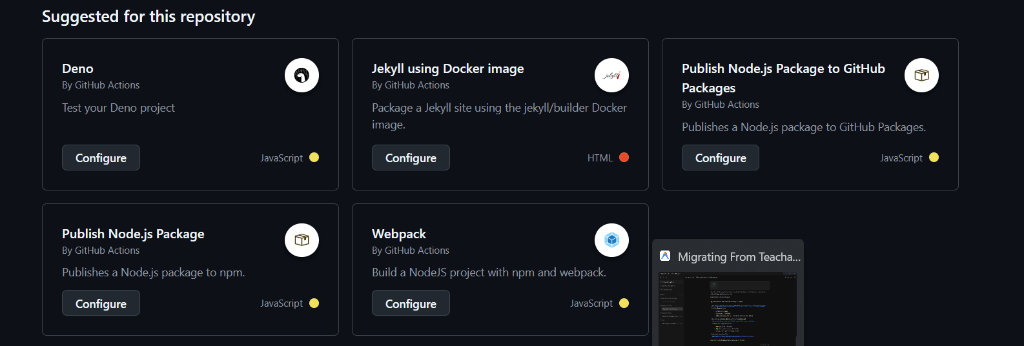
\includegraphics[width=1\textwidth]{images/ui-overview.png}
    \caption{Bảng tóm tắt các tính năng: Camera AI, Thống kê, Mạng xã hội và Quản lý thời gian}
\end{figure}

\subsection{3.5.2. Dashboard Thống kê và Biểu đồ Trực quan}
% CHÈN ẢNH VÀO ĐÂY
\begin{figure}[H]
    \centering
    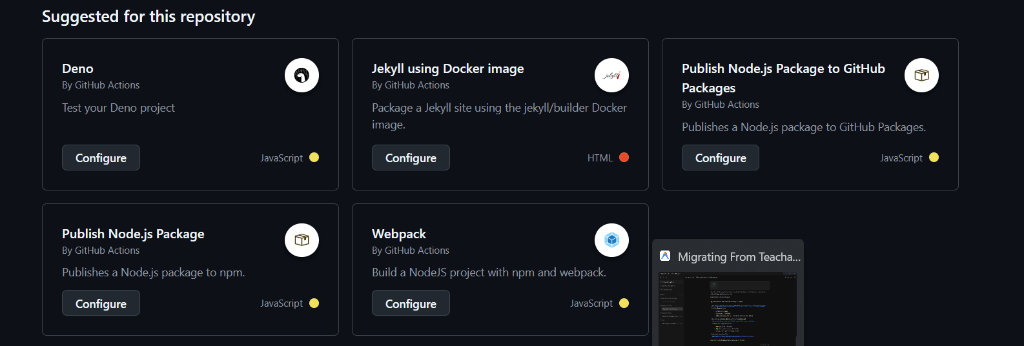
\includegraphics[width=1\textwidth]{images/ui-overview.png}
    \caption{Dashboard Thống kê phân bổ tư thế và Nhật ký theo thời gian thực}
\end{figure}

\subsection{3.5.3. Giao diện Mạng xã hội, Nhiệm vụ và Chat Box}
% CHÈN ẢNH VÀO ĐÂY
\begin{figure}[H]
    \centering
    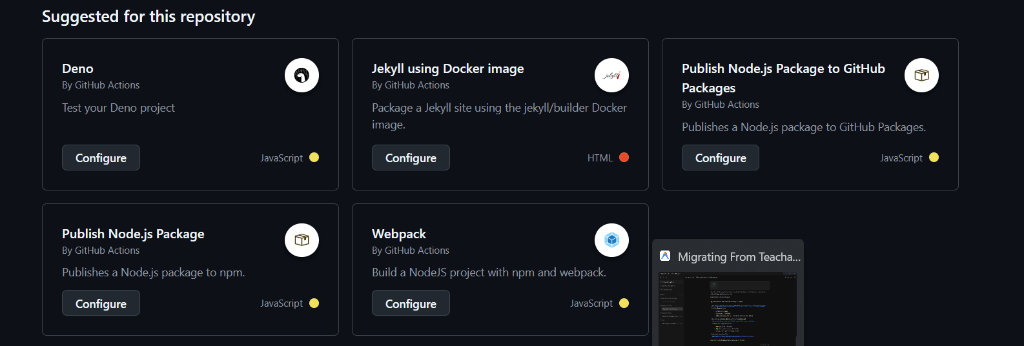
\includegraphics[width=1\textwidth]{images/ui-overview.png}
    \caption{Hệ thống Phòng học ảo (Chat) và Đồng hồ Pomodoro, Nhiệm vụ hàng ngày}
\end{figure}


% ==================== CHƯƠNG 4 ====================
\chapter{KẾT LUẬN VÀ HƯỚNG PHÁT TRIỂN}

\section{4.1. Đánh giá Ưu điểm nổi bật}
Trải qua toàn bộ quy trình từ khâu nghiên cứu thiết kế kiến trúc, cho tới việc code thủ công hoàn thiện hệ thống, dự án \textbf{PoseAlert} đã khẳng định được tính ứng dụng to lớn. Vượt qua giới hạn của một bài tập lớn lập trình thông thường, ứng dụng sở hữu những sức mạnh tiệm cận sản phẩm thương mại:

\begin{itemize}
    \item \textbf{Phá vỡ giới hạn bảo mật (Privacy Absolute):} Khác biệt cốt lõi nhất của PoseAlert là sự "Cứng rắng" trong việc bảo vệ dữ liệu người dùng. Máy ảnh chỉ "nhìn" chứ không hề "ghi". Mô hình Edge AI chạy tính toán bằng WebGL thẳng tại GPU của khách, giúp camera không bao giờ tiết lộ khung cảnh riêng tư ra ngoài thế giới Internet.
    \item \textbf{Triệt tiêu độ trễ (Zero Latency Processing):} Việc gửi video lên máy chủ (Server-side AI) mất hàng nghìn ms do độ trễ truyền dẫn (Ping). Trái lại, xử lý Client-side ở PoseAlert đưa tốc độ khung hình lên mức FPS trơn tru mượt mà ngay cả khi đứt cáp mạng.
    \item \textbf{Khả năng mở rộng (Infinite Scalability):} Nhờ kiến trúc Serverless, dự án hoàn toàn không có máy chủ nhận diện trung tâm. 10 người dùng hay 10 triệu người dùng cùng lúc, tốc độ xử lý AI không thay đổi. Trọng trách tính toán đã được đẩy sang hàng triệu thiết bị người dùng cá nhân (Distributed Computing).
    \item \textbf{Sinh thái Khép kín:} Sự hòa trộn giữa AI Y tế, Xã hội hóa (Chat) và Trò chơi hóa (Nhiệm vụ, Điểm thưởng) mang đến cho sinh viên một công cụ giải quyết tận gốc tính trì hoãn (Procrastination) và giữ gìn xương khớp.
\end{itemize}

\section{4.2. Những điểm Hạn chế (Limitations)}
Với tinh thần khoa học khách quan, dự án vẫn còn gặp rào cản mang tính giới hạn vật lý của kỹ thuật 2D Image Processing:
\begin{itemize}
    \item \textbf{Hiện tượng tắc nghẽn khớp (Occlusion):} Khi một bộ phận (VD: cánh tay) che khuất điểm khác (VD: hông), mô hình MoveNet đôi khi đưa ra phán đoán nhầm lẫn với độ tin cậy thấp, gây rung giật điểm neo (Jittering).
    \item \textbf{Mù chiều sâu (Lack of Depth):} Sử dụng camera 2D phẳng khiến thuật toán không thể nhận diện được bệnh gù lưng (Cụp vai ra phía trước) khi nhìn trực diện. Điều này chỉ có thể giải quyết nếu dùng thuật toán xoay 3D hoặc cảm biến chiều sâu (LiDAR/TrueDepth).
    \item \textbf{Sự phụ thuộc vào môi trường (Lighting constraints):} Ánh sáng trong phòng quá mờ hoặc người dùng ngồi ngược sáng (Backlight window) sẽ khiến độ chính xác của AI giảm mạnh do độ tương phản màu sắc biến mất.
\end{itemize}

\section{4.3. Định hướng Phát triển và Mở rộng tương lai (Roadmap)}
Nếu đề tài được tạo điều kiện để tiếp tục đầu tư và thương mại hóa, dưới đây là những nâng cấp chiến lược (Strategic Upgrades) sẽ được tiến hành:
\begin{enumerate}
    \item \textbf{Tích hợp 3D Pose Estimation (MediaPipe BlazePose):} Chuyển đổi công nghệ lõi sang phân tích hình thể theo trục chiều sâu (Z-axis). Nó sẽ mô phỏng tư thế bằng hệ xương góc khối (Kinematics), phân tích chi tiết được đường cong sinh lý của cột sống.
    \item \textbf{Hệ thống Hiệu chỉnh Cá nhân (Auto Calibration Setup):} Bổ sung bước thiết lập ban đầu (Onboarding). Hệ thống sẽ yêu cầu người dùng ngồi đúng tư thế chuẩn, chụp một bức ảnh khung xương đó làm "Chìa khóa gốc". Các cảnh báo sai tư thế sau này sẽ dựa trên việc đo mức độ sai lệch so với chính "khung xương chuẩn" của cá nhân đó, thay vì dùng một con số ngưỡng cố định, giúp cá nhân hóa độ chính xác lên 99\%.
    \item \textbf{Tích hợp AI LLM Khuyến nghị Y tế (AI Health Assistant):} Sử dụng các mô hình Ngôn ngữ lớn (Large Language Models) dạng API. Cuối mỗi tuần, AI Chatbot tự động đọc bảng dữ liệu Session của người dùng, đưa ra lời khuyên bằng văn bản và đính kèm các Video hướng dẫn tập Yoga/Dãn cơ cổ phù hợp.
    \item \textbf{Mở rộng hệ sinh thái ứng dụng di động:} Đóng gói nhân AI bằng React Native để đưa lên nền tảng App Store / Google Play, biến điện thoại di động thành thiết bị theo dõi sức khỏe thứ hai (Second-screen monitor).
\end{enumerate}

% ==================== NGUỒN THAM KHẢO ====================
\newpage
\chapter*{NGUỒN THAM KHẢO}
\addcontentsline{toc}{chapter}{NGUỒN THAM KHẢO}

\begin{enumerate}[label={[\arabic*]}]
    \item \textbf{Google TensorFlow Team (2021).} \textit{Next-Generation Pose Detection with MoveNet and TensorFlow.js.} Nguồn: \url{https://blog.tensorflow.org/2021/05/next-generation-pose-detection-with-movenet-and-tensorflowjs.html}.
    
    \item \textbf{Kho lưu trữ mã nguồn TensorFlow.js.} \textit{Pose Detection API}. Github. Nguồn: \url{https://github.com/tensorflow/tfjs-models/tree/master/pose-detection}.
    
    \item \textbf{Tài liệu kỹ thuật Google Firebase.} \textit{Firebase Realtime Database, Authentication \& Storage Docs}. Nguồn: \url{https://firebase.google.com/docs}.
    
    \item \textbf{Chart.js Contributors.} \textit{Chart.js Documentation - Simple yet flexible JavaScript charting for designers \& developers}. Nguồn: \url{https://www.chartjs.org/docs/latest/}.
    
    \item \textbf{Wikipedia.} \textit{Pomodoro Technique - Time Management Method}. Nguồn: \url{https://en.wikipedia.org/wiki/Pomodoro_Technique}.
    
    \item \textbf{Cao, Z., Hidalgo, G., Simon, T., Wei, S. E., \& Sheikh, Y. (2019).} \textit{OpenPose: realtime multi-person 2D pose estimation using Part Affinity Fields.} IEEE transactions on pattern analysis and machine intelligence, 43(1), 172-186.
    
    \item \textbf{World Health Organization (WHO).} \textit{Musculoskeletal conditions}. Nguồn: \url{https://www.who.int/news-room/fact-sheets/detail/musculoskeletal-conditions}.
\end{enumerate}

\end{document}
